\documentclass[12pt,a4paper]{article}
\usepackage[margin=2.5cm]{geometry}
\usepackage{helvet}
\renewcommand{\familydefault}{\sfdefault}
\usepackage[helvet]{sfmath}
\usepackage{amsmath,amssymb}
\usepackage{enumitem}
\usepackage{titlesec}
\usepackage{graphicx}
\usepackage{hyperref}
\usepackage[parfill]{parskip}
\usepackage{siunitx}
\usepackage{graphicx}
\graphicspath{{figures/}}

\providecommand{\seclabel}[1]{\label{sec:#1}}
\providecommand{\secn}[1]{Sec.~\ref{sec:#1}}
\providecommand{\figlabel}[1]{\label{fig:#1}}
\providecommand{\figr}[1]{Fig.~\ref{fig:#1}}
\providecommand{\pRef}{p_\mathrm{ref}}

\title{How Loudspeaker Impulse Responses Become Sound~Pressure~Level~(SPL) Plots:\\[0.7em]\textit{The Good, the Bad, and the Ugly}}
\author{Matthias S.~Brennwald}
\date{Document version \today}

\begin{document}
\maketitle

\section{Introduction}

Every loudspeaker designer or tinkerer wants to know how well their loudspeaker performs acoustically. Does it reproduce all frequencies evenly, or does it emphasise some and hide others? The answer lies in its SPL frequency response curve, which shows how loud the speaker is at each frequency.

Understanding and visualising the SPL response is central to almost every aspect of loudspeaker design and evaluation—from developing new drivers to characterising enclosures and interpreting room interactions. The goal seems simple: determine how a loudspeaker responds to different frequencies. The challenge lies in doing so accurately and efficiently, without (unintended) cheating.

An intuitive approach to determine the SPL curve of a loudspeaker would be to play a sine wave with a given frequency at a time, measure the resulting sound pressure level (SPL), repeat the process at the next frequency, and plot the SPL results across frequency. However, this method is very time-consuming and works reliably only in an anechoic environment, as room reflections and echoes can severely distort the measurement. Modern techniques achieve the same result in a single measurement step: they excite the loudspeaker with a short, broadband signal and use the Fourier transform to reveal the frequency response from the measured time-domain data.

This document introduces the concepts that link time-domain measurements (such as impulse responses) to frequency-domain data (such as SPL curves). It aims to provide a practical, intuitive explanation of what the Fourier transform does for loudspeaker measurements—and why understanding its limitations is just as important as applying it. Later sections explore both the strengths and the pitfalls of this process: the good, the bad, and occasionally the ugly.


\section{Time domain vs.\ frequency domain: the Fourier transform}\seclabel{Fourier_Theory}

Consider a sound pressure signal evolving as a function of time, $x(t)$. The signal is recorded by a microphone and digitized by an A/D converter with sampling rate \(F_s\). As a result, we obtain $N$ discrete samples $x_i = x(t_i)$ at times
\[
t_i = (i-1) \times \tau, \qquad \tau = \frac{1}{F_s}, \quad i = 1, 2, \ldots, N.
\]

The idea of the Fourier transform is to describe each time-domain data point \(x_i\)
as a combination of sine waves, each with amplitude \(A_j\) and phase \(\varphi_j\),
at discrete frequencies
\[
f_j = \frac{F_s}{N}j, \quad j = 1, 2, \ldots, M,
\]
where \(M = (N - 1)/2\) if \(N\) is odd, or \(M = N/2 - 1\) if \(N\) is even.

The discrete Fourier expansion is then written as:
\begin{align}
\text{For odd } N:\quad
x_i &= A_0 + \sum_{j=1}^{M} A_j \cos\!\big(2\pi f_j t_i + \varphi_j\big), \\[6pt]
\text{For even } N:\quad
x_i &= A_0 + \sum_{j=1}^{M} A_j \cos\!\big(2\pi f_j t_i + \varphi_j\big)
      + A_{N/2}\cos\!\big(\pi\, t_i / \tau\big).
\end{align}

Each amplitude–phase pair \((A_j, \varphi_j)\) represents one Fourier component at frequency \(f_j = jF_s/N\). The $A_0$ coefficient is the DC component of the $x_i$ data. Note that the total number of coefficients $A_j$ (including $A_0$) and $\varphi_j$ together equals \(N\). In other words, the number of data points in the frequency domain is the same as in the time domain. The above equations therefore represent a fully determined system. The coefficients \((A_j, \varphi_j)\) can be uniquely obtained from the measured samples \(x_i\) by solving this system, typically using efficient numerical algorithms such as the
\emph{Fast Fourier Transform (FFT)}.

Note that the Fourier transform is fully reversible. Given the frequency-domain data \((A_j, \varphi_j)\), the corresponding time-domain signal \(x_i\) can be reconstructed exactly using the same equations.  
In other words, the time-domain data describe how the signal evolves over time, while the frequency-domain data represent the same signal in terms of its amplitude and phase distribution across frequencies. Both domains contain precisely the same information; they are simply two equivalent representations of the very same signal.

\subsection{Periodic signals!}
An important (but often overlooked) aspect of the discrete Fourier transform is that it implicitly assumes the signal to be periodic with period $T = N \time \tau$.  
This follows directly from the use of sinusoidal functions, which are themselves periodic.  
In other words, when representing the discrete time-domain data $x_i$ as a sum of sinusoidal waves, the discrete Fourier transform assumes that this pattern repeats indefinitely for $t < 0$ and $t > T$.  
However, in many practical cases the measured signal is not actually periodic—for example, the impulse response discussed in \secn{impulse_response}.  
This assumption is not inherently a problem, but it does have consequences: if the start and end points of the time-domain data are not at the same amplitude, the implied periodic continuation introduces an artificial discontinuity at the boundary between repetitions.  
In the frequency domain, that discontinuity appears as additional spectral content (spectral leakage).

\subsection{Where did the other frequencies go?}
In practice, most real-world signals are not composed of a finite set of perfectly aligned frequencies $f_j$.  
Instead, their spectral energy almost always lies between the discrete frequencies sampled by the Fourier transform.

In the discrete Fourier transform, the available frequencies form equally spaced bins centered at the $f_j$, each with width $\Delta f = F_s/N = F_s \times \tau$.
A signal whose frequency does not coincide with one of these discrete $f_j$ values will have its energy distributed over multiple bins, a phenomenon known as spectral leakage. While the total energy of the signal remains conserved, leakage can cause sharp spectral features to appear broadened or blurred across multiple frequency bins.

Sampling also imposes two important frequency limits.  
The lowest frequency present in the discrete Fourier transform ($f_1 = F_s/N$) is determined by the total length of the digitized signal, $T = N \times \tau$.  
Because the bin width $\Delta f$ equals $f_1$, the signal duration also defines the frequency resolution of the time-domain data.  
The highest resolvable frequency ($f_M = F_s \times M / N$) is determined by the sampling rate: according to the Nyquist theorem, no frequency above $F_s/2$ can be represented in the digitized data.  
Any analog signal components above this limit will be folded back (or ``aliased'') to appear as spurious lower-frequency components in the sampled data.


\section{The impulse response and its Fourier transform}\seclabel{impulse_response}
Imagine a test signal that contains all frequencies at once, each with the same amplitude and zero phase; that is, $A_j = 1$ and $\varphi_j = 0$ for all $j = 1, \ldots, M$. The DC component is $A_0 = 1$ and, for even $N$, the Nyquist component is $A_{N/2} = 1$. When such a signal is converted from the frequency domain to the time domain, the result is a very short pulse at time $t_1$ and zero at all other times $t_{i = 2\ldots N}$ -- a Dirac delta. In other words, an ideal Dirac pulse excites all frequencies simultaneously, with equal amplitude and phase.

If we now drive a loudspeaker with this impulse, the microphone records its acoustic output over time.  
The resulting waveform, $h(t)$, is the impulse response, expressed in sound pressure (Pa) as a function of time.  
Because the input contains all frequencies equally, any variation in the measured response reflects how the loudspeaker modifies the amplitude and phase of those frequencies, revealing its deviation from a perfectly flat response.

The impulse response thus captures the complete acoustic behaviour of the loudspeaker (and the surrounding room): every resonance, reflection, and delay leaves its fingerprint in $h(t)$.  
Early peaks correspond to the direct sound from the driver, later ripples often indicate cabinet or cone resonances, and delayed arrivals show reflections from walls or nearby objects.


\section{The impulse response and its Fourier transform}

Imagine a test signal that contains all frequencies at once, each with the same amplitude and zero phase; that is, $A_j = 1$ and $\varphi_j = 0$ for all $j = 1, \ldots, M$, together with a DC component $A_0 = 1$ (and for even $N$, a Nyquist component $A_{N/2} = 1$). When such a spectrum is converted from the frequency domain to the time domain using the above Fourier expansion, the result is $x_1 = N$ and $x_{i=2\ldots N} = 0$, the discrete analogue of a Dirac delta. In other words, an ideal delta pulse contains all frequencies simultaneously and with equal amplitude and zero phase.

If we now drive a loudspeaker with this impulse, the microphone records its acoustic output over time ((\figr{FIGURE1}).  
The resulting waveform, $h(t)$, is the impulse response, expressed in sound pressure (Pa) as a function of time (\figr{FIGURE1}-B). Because the input contains all frequencies equally, any variation in the measured response reflects how the loudspeaker modifies the amplitude and phase of those frequencies—revealing its deviation from a perfectly flat, ideal response.\footnote{In practice, a very large impulse is required to achieve a good signal-to-noise ratio of the measurement. Most measurement tools therefore do \emph{not} use a Dirac impulse to determine the impulse-response, but rely on maximum-length sequences, broadband noise, or sine sweeps to excite the loudspeaker. The recorded loudspeaker response is the deconvolved from the test signal to obtain the impulse response. The result is the same as in our thought experiment, but with less measurement noise.}

Imagine the measurement of the impulse response were carried out in an anechoic environment. The resulting impulse response would capture the complete acoustic behaviour of the loudspeaker (\figr{FIGURE1}-B): every resonance, reflection, and delay leaves its fingerprint in $h(t)$. Early peaks correspond to the direct sound from the driver, and later ripples often indicate cabinet or cone resonances, which at some point dye off in the noise floor of the measurement.

In practice, however, measurements usually cannot be carried out in a perfectly anechoic environment. The sound radiated from the speaker gets reflected at the floor, the ceiling and the walls of the room, and furniture or other objects. These reflections show up in the measurement as small wiggles after the main peak of the direct sound from the speaker (\figr{FIGURE1}-C).

\begin{figure}[tbp]
  \begin{center}
    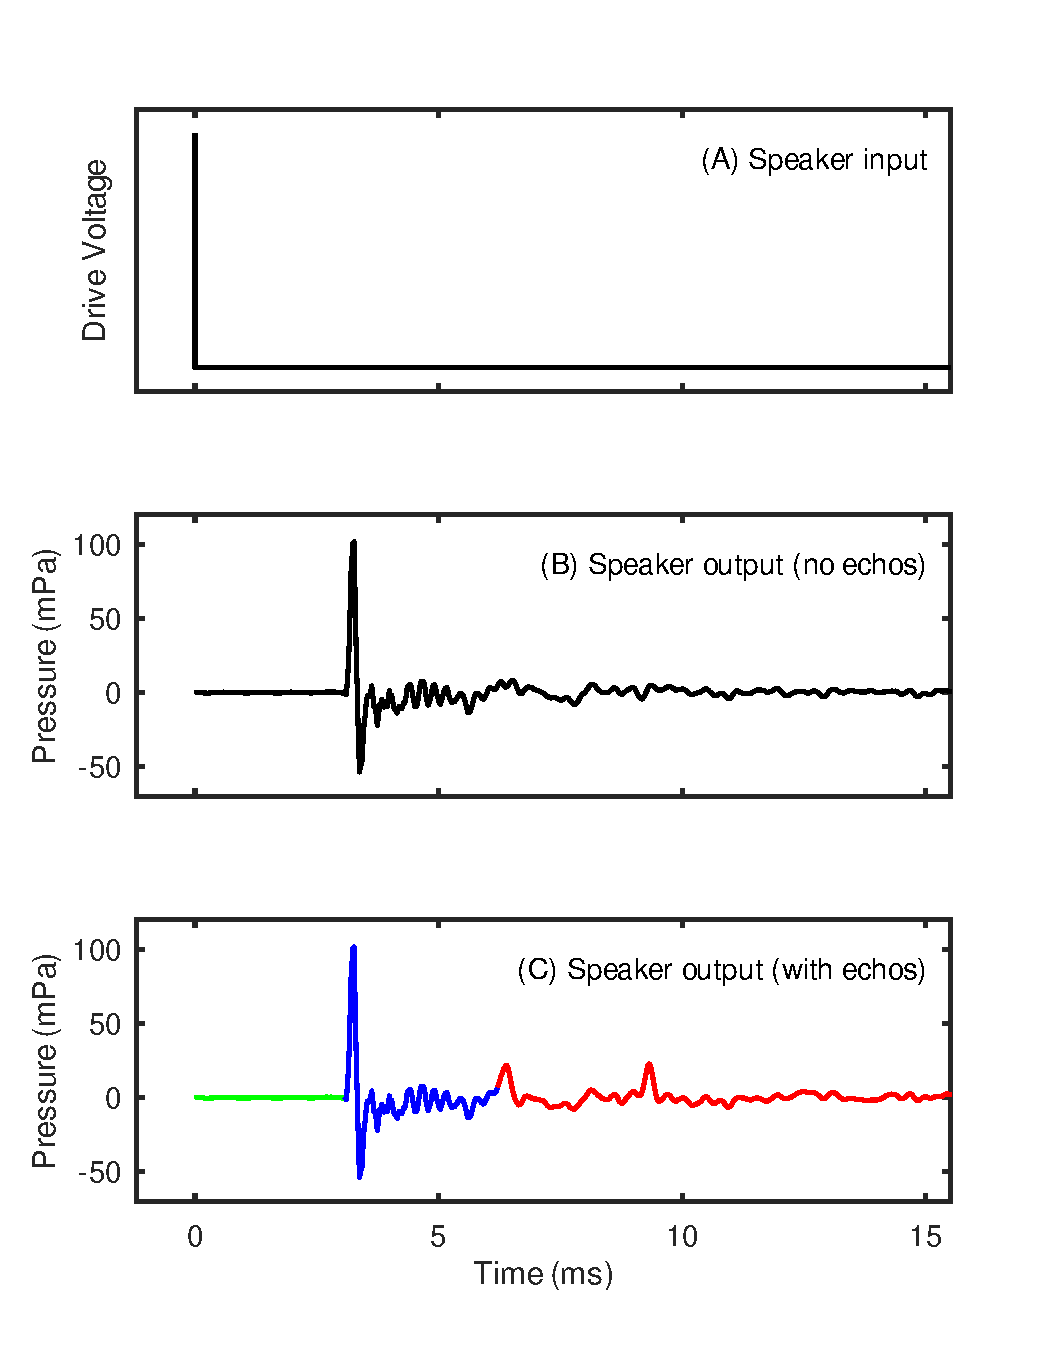
\includegraphics[width=0.7\textwidth]{FIGURE1}
    \caption{Loudspeaker impulse response. (A) The Dirac signal input to the loudspeaker, (B) loudspeaker impulse response in an anechoic environment (which is usually not accessible with a typical measurement setup), (C) impulse response of the same loudspeaker, but from a more typical measurement setup resulting in echos from the room walls.}
    \figlabel{FIGURE1}
  \end{center}
\end{figure}

\section{From impulse response to the SPL curve: gating (reality bites!)}

We have seen how a single measurement of the impulse response contains everything needed to determine a loudspeaker’s acoustic behaviour.
But, before applying the Fourier transfor to the time-domain measurement, let's take a closer look at \mbox{\figr{FIGURE1}-C}:
\begin{itemize}
\item The beginning of the impulse-response measurement (green, 0--\SI{3.08}{ms}) represents the flight time of the sound from the loudspeaker to the microphone and contains no useful information about the loudspeaker itself.
\item The initial part of the impulse response (blue, 3.08--\SI{6.23}{ms}) shows the clean, direct sound from the loudspeaker.
\item After the arrival of the first echo at \SI{6.23}{ms}, the direct signal becomes masked by reflections from the room.
This echoic part of the signal (red) still contains the loudspeaker’s output, but it can no longer be used to assess the loudspeaker’s own behaviour.
\end{itemize}

Only the anechoic segment of the impulse response can therefore be used to characterise the loudspeaker’s behaviour under anechoic conditions. The flight-time and echoic parts of the impulse-response measurement are discarded. In other words, the impulse response is gated to its anechoic part. The Fourier transform of this gated impulse response then yields the amplitude coefficients $A_j$, and hence the loudspeaker’s clean, anechoic SPL data in units of dB-SPL:
\[
\mathrm{SPL}(f_j) = 20 \log_{10}\left( \frac{A_j / \sqrt{2}}{\pRef} \right)
\]
where $\pRef = \SI{20}{\micro\pascal}$ is the SPL reference pressure.

\figr{FIGURE2} shows the SPL data determined from the anechoic part of the impulse response shown in \figr{FIGURE1}. The number of time-domain data points in the anechoic segment is $N = 140$. The frequency-domain data contains the same number of data points, split between amplitude ($A_j$) and phase ($\varphi_i$) coefficients (see \secn{Fourier_Theory}). The anechoic time-domain segment is $T = \SI{3.15}{ms}$ long, so the lowest frequency ($f_1$) and the width of the frequency bins ($\Delta f$) determined as $1/T \approx \SI{317}{Hz}$. The ``rough'' presentation of the SPL data in \figr{FIGURE2} may seem awkward, but it clearly exposes the limits of the method with respect to the low-frequency extension and frequency resolution (bin width) of the SPL data.

\begin{figure}[tbp]
  \begin{center}
    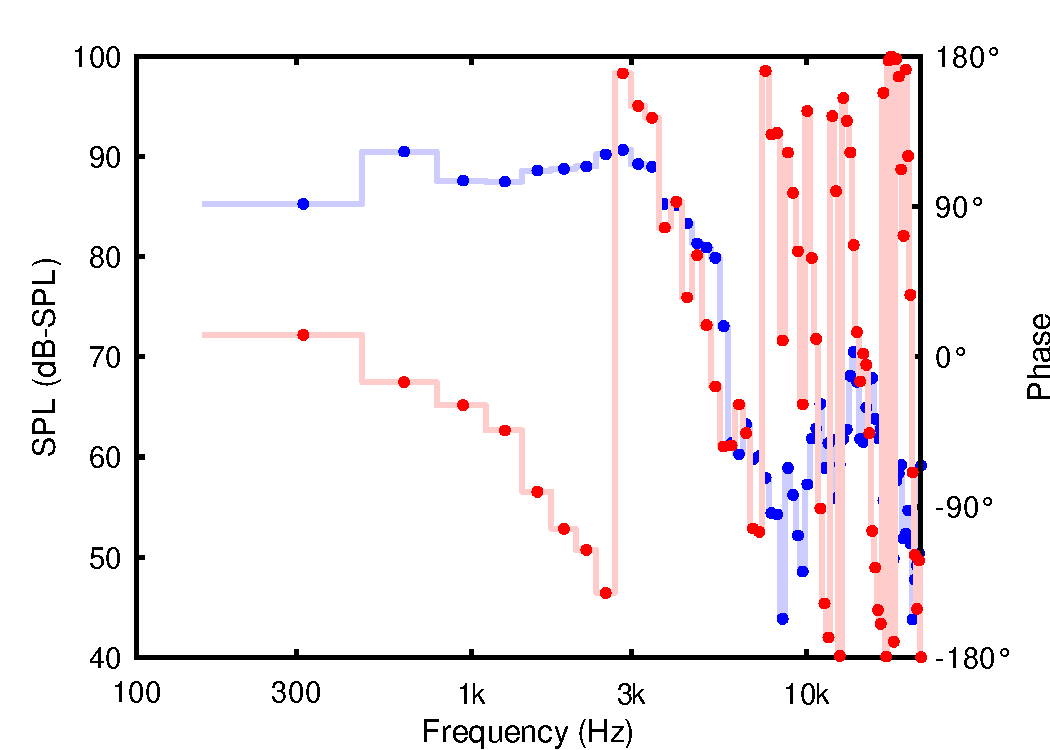
\includegraphics[width=0.7\textwidth]{FIGURE2}
    \caption{SSPL data determined from the anechoic part of the impulse response in \figr{FIGURE1} (see text). The dots show the frequency-domain data ($\mathrm{SPL}(f_j)$ and $\varphi_j$). The stair steps indicate the frequency bin width ($\Delta f$), which is constant across the entire plot but appears distorted due to the logarithmic scaling of the frequency axis.}
    \figlabel{FIGURE2}
  \end{center}
\end{figure}

The following sections discuss some commonly used techniques used to tweak the anechoic data or to make it look prettier -- but remember: \emph{looks can be deceiving!}


\section{Dealing with reality: The Good, the Bad, and the Ugly}
DISCUSS THE METHODS INTRODUCED IN PREVIOUS SECTIONS, DEMONSTRATE THEIR (AB)USE AND EFFECTS 

% The relationships described in \secn{Fourier_Theory} define the discrete time and frequency grid on which the Fourier transform operates. Real-world signals rarely align perfectly with this grid, which is why techniques to reduce leakage or to improve the visual appearance of and SPL curve are applied -- sometimes for the better, sometimes not.

\subsection{Low-frequency extension and frequency-resolution of the SPL curve}
DISCUSS HERE. LF LIMIT $f_1$ and BIN WIDTH $\Delta f$.


\subsection{Is the gated impulse response periodic?}
DISCUSS HERE. WINDOW FUNCTIONS TO FORCE PERIODIC SIGNAL. attenuates/messes the tail of the impulse response, so data is changed or lost.



\begin{itemize}[noitemsep]
    \item The following sections discuss how real-world processing shapes this transformation:
    \begin{itemize}
        \item \textbf{The Good:} gating and windowing to suppress reflections.
        \item \textbf{The Bad:} excessive windowing that removes low-frequency content.
        \item \textbf{The Ugly:} manipulation of data through zeroing, smoothing, or padding.
    \end{itemize}
    \item Each step is an attempt to recover the true loudspeaker behaviour from a reflection-rich environment—but not all are equally honest.
\end{itemize}

\vspace{1em}
\noindent\rule{\textwidth}{0.4pt}\\
\textit{This conceptual introduction explains how an impulse response represents a complete description of a loudspeaker’s behaviour. Later sections explore how this data is processed, interpreted, and occasionally abused.}

\end{document}
